\documentclass{ecnreport}

\stud{EMARO-ARIA}
\topic{Advanced Robot Programming}

\begin{document}

\inserttitle{Advanced Robot Programming  Labs \newline C++ Programming}

\insertsubtitle{Lab 1: Open projects}

\newcommand{\involves}[1]{
\item {\bf C++ skills:} #1
}

\newcommand{\aitip}[1]{
\item {\bf AI tips:} #1
}


\section{Content of this lab}

The goal of the first C++ labs is to discover the language by building small projects.
Many projects are listed below and you are encouraged to try and build several of them. Most of them can be done without using evolved concepts of C++. You can also build your own project if you have a clear idea of the goal to be reached.\\

You are encouraged to use functions, classes or even templates if you think it will lead to a better code that is easier to understand and to write.
You are also encouraged to separate your code in several files. If you are not sure about classes or functions, you can always change it later and compare
the same program with different code designs.\\

You may look for mathematical solutions, problem formulation or problem variations on Internet, but of course the actual code should come from yourselves. \\

These problems can also be used to learn other programming languages. Other exercices and challenges can be found online:
\begin{itemize}
\item https://www.codingame.com : program smalls games online and visualize what you do
\item https://codefights.com : solve small to large problems online, compare your code with other participants
\end{itemize}

\subsection{How to compile}

We use CMake tools to compile our projects.
The content of the CMakeLists.txt file should follow the structure of your code directory (or preferably sub-directory):
\begin{center}
\begin{minipage}{.4\linewidth}
 \dirtree{%
.1 MyProject. 
.2 include.
.3 a\_class.h.
.3 some\_functions.h.
.3 a\_basic\_header.h.
.2 src.
.3 main.cpp.
.3 a\_class.cpp.
.3 some\_functions.cpp.
.2 CMakeLists.txt.
} 
\end{minipage}
\begin{minipage}{.55\linewidth}\pythonstyle
\begin{lstlisting}
cmake_minimum_required (VERSION 2.6)
project (MYPROJECT)

add_compile_options(-std=c++11)

include_directories(include)

add_executable(mygame 
  src/main.cpp include/a_basic_header.h
  include/a_class.h a_src/class.cpp
  include/some_functions.h src/some_functions.cpp)
\end{lstlisting} \end{minipage}
\end{center}

The CMake file is used to generate a Makefile. The steps are:
\begin{enumerate}
 \item Create a build directory: \texttt{mkdir build}
 \item Go inside: \texttt{cd build}
 \item Call CMake: \texttt{cmake ..}
 \item Call Make: \texttt{make}
 \item Then launch your program: \texttt{./mygame}
\end{enumerate}

\subsection{How to use QtCreator}

The IDE\footnote{Integrated Development Environment} that will be used for C++ (and all my other labs) is Qt Creator. It is an open source, multi-platform IDE based on the Qt framework (which is used in the KDE Linux desktop). 
Before loading a project in Qt Creator, you have at least to write a basic CMakeLists.txt file (even without executables) and to create the \texttt{build} folder. You can then run Qt Creator:
\begin{enumerate}
\item Load the CMakeLists.txt file through \texttt{File...open project}
\item Give the path to your \texttt{build} directory
\item Qt Creator will then execute CMake and display the source files found in CMakeLists.txt (if any)
\item To add a file (.cpp or .h), you can create an empty one with \texttt{File... new file} 
\item Add this file in the CMakeLists.txt and right-click on the Project to run CMake to tell Qt Creator that the structure of the project has changed
\item Compilation is done by clicking the bottom-left hammer
\item Run your program with the green triangle. However, if you need user input, you will need to run the program from the console.
\item Do to so, open a terminal, go to the \texttt{build} folder and type the name of the program: \texttt{./myprogram}
\end{enumerate}


\section{Single player games}

In the single player games, the opponent is the computer which plays with a basic or advanced AI depending on your programming
motivation (and game AI possibilities...).


\subsection{Find the number}

Here the computer start by choosing randomly a number between 1 and 100. The player has to find this number with trial and error, the only answer being whether the number is greater or lesser than the goal.
This can also be done in reverse, where the computer has to guess.

\begin{itemize}
 \involves{Input/output}
 \aitip{Random numbers depend on seed}
\end{itemize}

\subsection{Rock-paper-scissors}

The player is asked to choose between rock, paper or scissors. The computer also does a choice and the winner depends on the two choices: Rock beats Scissors, Paper beats Rock, Rock beats Scissors, Draw in the case of equal choices.

\begin{itemize}
 \involves{Input/output, Random numbers}
  \aitip{none, this game is completely random}
\end{itemize}

\section{Turn-based text games}

In these two-player games, the players play one at a time. The goal is usually to reach the winning situation before the other.
They can also be programmed to play against an artificial intelligence. This time the AI can be much more complex than for the first games.

\subsection{21 sticks game}

In this game, a given umber of sticks (typically 21) are displayed.
Each player has to pick up 1 to 3 sticks, then the other player can pick up his sticks.
The goal is not to have to pick the last stick.

\begin{itemize}
 \involves{Input/output}
 \aitip{If you can start correctly you may never lose}
\end{itemize}

\subsection{Battleship}

In this game each player has a number of boats that are placed on a 10$\times$10 grid. The goal is to sink all the opponent's boats.
Each player begins by placing their boats according to the following:
\begin{itemize}
 \item One Aircraft carrier [A] of length 5
 \item One Cruiser [C] of length 4
 \item One Destroyer [D] of length 3
 \item One Submarine [S] of length 3
 \item One Minesweeper [M] of length 2
\end{itemize}

The player grids may be entered manually or with a text file (check grid consistency), or randomly generated.
Each player then enters coordinates of the targeted grid cell. A boat can be hit, sunk or it may be a miss. 

The current grids should be displayed with:
\begin{itemize}
 \item A dot for a non-targeted cell
 \item A cross for missed shots
 \item The boat letter for hit or sunk boats
\end{itemize}

\begin{center}
 \begin{tabular}{|c|c|c|c|c|c|c|c|c|c|c|}
 \hline 
 & 0 & 1 & 2& 3&4 &5 &6 & 7&  8&9 \\\hline
 0 &x&.&.&. &.& .&.&.&.&.\\\hline
 1 &.&.&.&. &C&C&x&.&.&.\\\hline
 2 &.&x&.&. &.&.&.&M&.&.\\\hline
 3 &.&.&.&. &.&.&.&.&.&.\\\hline
 4 &.&.&.&. &.&.&.&.&.&.\\\hline
 5 &.&.&x&. &A&A&A&A&A&.\\\hline
 6 &.&.&.&. &.&.&.&.&.&.\\\hline
 7 &.&.&.&. &.&.&.&.&.&.\\\hline
 8 &.&.&.&. &.&.&.&x&.&.\\\hline
 9 &.&.&.&. &.&.&.&.&.&.\\\hline
 \end{tabular}
\end{center}
\begin{itemize}
 \involves{Input/output, Vectors, File input, Data representation}
 \aitip{Do not target the same cell twice, finish what you started}
\end{itemize}


\subsection{4 in a row}

This game is played on a 6$\times$7 grid. Each player has to drop a token in one of the column, that will fall to the bottom or above potential existing tokens in this column.
The goal is to be the first to align 4 tokens, either vertically, horizontally or diagonally.

\begin{center}
 \begin{tabular}{|c|c|c|c|c|c|c|}
 \hline  
 . &.&.&.&. &.&.\\\hline
 . &.&.&.&. &.&.\\\hline
 . &.&.&.&. &.&.\\\hline
 . &.&.&.&. &.&.\\\hline
 . &.&o&.&x &.&.\\\hline
 . &o&x&x&o &o&.\\\hline
 \end{tabular}
\end{center}
\begin{itemize}
 \involves{Input/output, Vectors, Data representation}
 \aitip{Do not let the other player align 4 token (that is just trying not to lose), or try to guess best possible choices for the next 1, 2, 10... turns.}
\end{itemize}

\newpage

\section{Algorithms}

In this section, we program the computer to solve a given problem through an algorithm. Similarly to a cooking recipe, an algorithm is a sequence of basic steps (like finding the minimum value in a vector) that lead to an overall more complex behavior.

The problem data may be defined in a file or be randomly generated.
The use of the STL and of the \texttt{math.h} functions will be of good use. 

\subsection{1D function minimization}

Function minimization consists in finding the minimum value of a function, and where this value is reached. A classical algorithm to do so is the gradient descent. The corresponding algorithm is as follow:

\begin{algorithm}[!h]
\SetKwComment{Comment}{(}{)}
% \SetAlgoLined
\KwData {derivative $f'$, starting point $x$, max iterations, gain $\lambda$, min gradient $g_m$}
\KwResult {$x$, the point where f reaches its minimum value}
%add $P_0$ to $\mathcal{P}_s$\;
iter$\gets$0\;
$g\gets2\times g_m$\;
\While{iter $<$ iter$_{max}$ and $g < g_m$}
{
$g\gets f'(x)$\;
$x\gets x - \lambda.g$\;
}
\Return $x$\;
\caption{Gradient descent}
\label{algo:grad}
\end{algorithm}

This algorithm relies on the function derivative $f'(x)$ that must be defined. A simple case can be to find the minimum of the function $f(x) = ax^2+bx+c$ where $a>0$, starting from any value of $x$.

\begin{itemize}
 \involves{Functions}
 \end{itemize}
 
\subsection{nD function minimization}

Here the function to be minimized is still a scalar but may take several arguments. A typical case is a quadratic function over $\mathbb{R}^n$: $f(\x) = \x^T\Q\x$. The algorithm is the same as in 1D minimization except that $\x$ has several components. Instead of a function for the derivative, we need thus a function to compute the Jacobian of $f$ that will return a n-D vector for all derivatives along the $x_i$'s. 

\begin{itemize}
 \involves{Functions, Vector}
 \end{itemize}

 
\subsection{Tower of Hanoi}

This one is a classical mathematical puzzle.
A given number of disks of different sizes are placed on three rods.
The only constraint is that a bigger disk cannot be above a smaller one. 

The goal is to move the disks one at a time (only the top disk of a rod may be moved to another rod) in order to have them all on a single rod.
The Wikipedia page will give you strong hints to solve this problem.

The starting position of the disks may be randomly generated or written in a file. The goal is of course to use a minimum number of moves.

\begin{itemize}
 \involves{File input, output, Vectors, Data representation, Recursive programming (functions)}
 \end{itemize}
 
 \subsection{Reachable numbers with only 6 6's}
 
 In this problem we are trying to write numbers with only 6 6's, as in:
 \begin{eqnarray*}
  1 =& 6/6 + 6 +6-6-6 \\
  2 =& 6/6 + 6/6 + 6 - 6 \\
  6 =& 6\times 6/6 + (6-6)/6 \\
  10 =& (6\times(6+6) -6 -6)/6
 \end{eqnarray*}
 All 4 operations $\{+, -, \times, /\}$ are allowed in any order and any priority.
 The goal is to find:
 \begin{enumerate}
  \item The first number that cannot be written this way.
  \item The number of numbers that can be written this way.
 \end{enumerate}
\begin{itemize}
 \involves{Functions, Recursive programming, Vectors}
 \end{itemize}
 
 
 \subsection{Robust fitting with Hough lines}
 
 This method will be taught in Computer Vision. We assume we have a number of $(x,y)$ points and want to find the line or lines that pass through them.
 A method was proposed by Hough and consists in finding all possible lines that pass through each point, and then count the similar lines. The ones that have
 the highest number of counts (or votes) are considered to be actual lines in the image.
 Do to so, we write a line equation as:
 \begin{equation*}
  x\cos\theta + y\sin\theta = \rho
 \end{equation*}We then consider a finite set of possible $\theta$ and $\rho$, typically:
 \begin{itemize}
  \item $\theta$ can go from $-\pi/2$ to $+\pi/2$ with 100 intermediary values
  \item $\rho$ can go from 0 to half the diagonal of the image with 100 intermediary values
 \end{itemize}
 We thus have a 100$\times$100 grid of all potential $(\rho,\theta)$ corresponding to 10000 lines.
 
 In practice, at the beginning of the program you can define $X$ as [-10, .., 10] and chose one, then two values for $(a,b)$.
 Then $Y$ is computed as $Y=aX+b$ and you have your set of X and Y coordinates. You can also add some random points to make it more difficult to the algorithm.
 
 The algorithm is given below.

 
\begin{algorithm}[!h]
\SetKwComment{Comment}{(}{)}
% \SetAlgoLined
\KwData {X and Y, min. votes n}
\KwResult {$(\rho,\theta)$ for best lines}
%add $P_0$ to $\mathcal{P}_s$\;
init $\rho_v$ and $\theta_v$ vectors from desired range and step\;
RT$\gets$zero matrix of dim. 100$\times$100\;
\For{i in range(100)}{
\For{(x,y) in (X,Y)}
{
$\rho\gets x\cos\theta_i + y\sin\theta_i$\;
j$\gets$index of $\rho_v$ nearest to $\rho$\;
RT[j,i]+= 1\;
}}
$(\rho,\theta)$ are the values where RT[i,j] $>$ n\;
\caption{Hough line detector}
\label{algo:hough}
\end{algorithm}

\begin{itemize}
 \involves{Output, Vectors, Sort and Find maximum (STL)}
 \end{itemize}
 
 
 
 
 \subsection{Path planning with A*}
 
 The A* algorithm is a popular path planning method that can easily find the shortest path from a starting to a desired position in a graph. 
 A graph is a set of nodes (positions or situations) linked by elementary steps (for example, going from (0,0) to (0,1)). It may be a classical 2D or 3D space, but
 also any kind of graph where we want to find the shortest path. 
 
 \begin{itemize}
 \involves{File input and output, Vectors, Data representation, Sort and find minimum (STL), Classes, Inheritance, Templates or References}
 \end{itemize}
 
 \subsubsection{General A* algorithm}
 The algorithm is based on two functions:
 \begin{itemize}
  \item The travel function $g(i)$ expresses the distance between the starting position and the evaluated one. 
  \item The heuristic function $h(i)$ tries to estimate the cost from the current position to the desired one. 
 \end{itemize}The total cost function is the sum of $g$ and $h$.
It is also using two sets of nodes:
\begin{itemize}
 \item The closed set regroups all nodes that have been evaluated (starts at empty)
 \item The open set regroups all nodes that are to be evaluated (starts with the initial position)
\end{itemize}


\begin{algorithm}[!t]
\SetKwComment{Comment}{(}{)}
% \SetAlgoLined
\KwData {start and goal positions}
\KwResult {Sequence of nodes that define the shortest path}
%add $P_0$ to $\mathcal{P}_s$\;
closedSet$\gets$ []\;
openSet$\gets$ [start]\;
start.g$\gets$ 0\;
start.compute\_h(goal)\;
start.compute\_f()\;
\While{openSet not empty}{
candidate $\gets$ node in openSet with lowest f score\;
\If{candidate == goal}{
return candidate\;}

openSet.remove(candidate)\;
closedSet.add(candidate)\;
\For{each neighboor of candidate}{
union$\gets$openSet + closedSet\;
\eIf{neighboor is in union}
{
twin$\gets$neighboor from union set \;
\If{twin.g $>$ neighboor.g}{
twin.set\_parent(candidate)\;
twin.compute\_f()\;
openSet.add(twin)\;
}
}
{
neighboor.compute\_h(goal)\;
neighboor.compute\_f\;
openSet.add(neighboor)\;
}
}

}
\caption{A* algorithm}
\label{algo:smallpoly}
\end{algorithm}

As we see, the algorithm does not depend on the type of the nodes, as long as the following can be defined:
\begin{itemize}
 \item The $h$ function from the node to the goal
 \item The $neighboor$ function that gives the nearest nodes to the current node (\texttt{vector}?)
 \item The $==$ operator that checks whether two nodes are the same
\end{itemize}

This is perfect for classes as the actual algorithm can be written in a generic way. I suggest you write it for a given class to test it without using templates.


\subsubsection{Classical 2D path planning}

This first A* problem consists of a 20$\times$20 grid where a robot must go from $(0,0)$ to $(19,19)$.
Obstacles exist of course in the grid. They can be defined randomly or in a text file that the program will read.
In this case:
\begin{itemize}
 \item The $h$ function is the Euclidean distance to the goal.
 \item The $neighboor$ function should give all the nodes reachable from a $\pm1$ move on x or y.
 \item The $==$ operator corresponds to having equal x and y.
\end{itemize}

\subsubsection{The 8-puzzle or 15-puzzle problem}

In this problem, we have a 3$\times$3 grid with cells numbered from 1 to 8\footnote{can also be done on a 4$\times$4 grid with numbers 1..15}, and an empty cell.
The goal is to reach the following configuration:
\begin{center}
 \begin{tabular}{|c|c|c|}
 \hline  
 1 &2&3\\\hline
 4 &5&6\\\hline
 7&8&.\\\hline
 \end{tabular}
\end{center}
We go from one position to another one by sliding one cell in the empty cell. For example, the two configurations that may lead to the desired one are:
\begin{center}
 
 \begin{tabular}{|c|c|c|}
 \hline  
 1 &2&3\\\hline
 4 &5&6\\\hline
 7&.&8\\\hline
 \end{tabular}\quad\quad\quad
 \begin{tabular}{|c|c|c|}
 \hline  
 1 &2&3\\\hline
 4 &5&.\\\hline
 7&8&6\\\hline
 \end{tabular}
\end{center}

In this case:
\begin{itemize}
 \item The $h$ function can be the Manhattan distance, that is:
 \begin{equation*}
  h(x,y) = \sum_{i=1}^8(|x_i - x_i^*| + |y_i - y_i^*|)
 \end{equation*}where $(x_i,y_i)$ is the position of cell $i$ in the grid and $(x_i^*,y_i^*)$ is the position
 of cell $i$ in the desired grid.
 \item The $neighboor$ function should give all the grids reachables from the current one.
 \item The $==$ operator corresponds to having the cells at the same positions.
\end{itemize}

Note that not all starting grids can reach the desired one. The best way to build a starting position is to start from the desired one and randomly move cells
for 30 to 40 steps. You will be surprised the algorithm will usually find a much shorter path to come back.

You should write the different steps in a file with the corresponding move and grid, to go from the starting grid to the desired one.

\subsection{Genetic algorithms}


Sometimes we want to find the minimum of a function that has many input variables and where the gradient descent algorithms cannot work because we have a lot of local minima (meaning that quickly the algorithm will stop even if the global minimum is not reached). In this case, Genetic Algorithms are a class of methods that are based on a heuristic search of the minimum. 

In the GA method, an input point is called an individual and has a given score (which is simply the function evaluated for this input). We start by generating a set of random individuals, called the population. We then keep a number of best individuals amongst this population, and fill up the new population by re-generating new individuals that may be better. The overall algorithm is represented in Algorithm \ref{algo:ga}.

As we see, the algorithm by itself only needs three particular functions for individuals:
\begin{itemize}
\item The evaluation function that gives the score of the individual.
\item The Crossing function that takes two individuals to return a new one. This function can be seen as changing two parents into one child that would be a mix of the parents's properties.
\item The Mutate function that slightly changes an individual.
\end{itemize}These functions depend on the actual problem that we are solving, two examples are shown below.

 \begin{itemize}
 \involves{File input and output, Vectors, Data representation, Sort and find minimum (STL), Classes, Inheritance, Templates or References}
 \end{itemize}

\begin{algorithm}[!h]
\SetKwComment{Comment}{(}{)}
% \SetAlgoLined
\KwData {Population size n, function $f$ to be minimized, max iterations that do not change the best individual, number k of individuals that we always keep}
\KwResult {Individual that minimizes $f$}
%add $P_0$ to $\mathcal{P}_s$\;
population$\gets$ n random individuals\;
iter$\gets$0\;
\While{iter $<$ iter$_{max}$}{
best$\gets$best individual from population\;
new\_population$\gets$best k individuals from population\;
\For{i from k+1 to n/2}{
n1$\gets$random number between 1 and n\;
n2$\gets$random number between 1 and n, different from n1\;
new\_population$\gets$ best between population[n1] and population[n2]\; 
}
\For{i from 1 to n/2}{
n1$\gets$random number between 1 and n\;
n2$\gets$random number between 1 and n, different from n1\;
new\_indiv = cross(population[n1], population[n2])\;
new\_indiv.mutate()\;
new\_population.Add(new\_indiv)\;
}
population$\gets$new\_population\;
new\_best$\gets$best individual from population\;
\eIf{new\_best == best}{iter$\gets$iter+1\;}{iter$\gets$0\;}
}
\caption{Genetic Algorithm}
\label{algo:ga}
\end{algorithm}\newpage
 
\subsubsection{Minimizing a function on $\mathbb{R}^2$}

A classical function to test GA is the Rastrigin's function:
\begin{equation*}
f(x,y) = 20 + x^2 + y^2 - 10\left(\cos(2\pi x) + \cos(2\pi y)\right)
\end{equation*}The graph looks like this, with the global minimum at (0,0):
\begin{center}
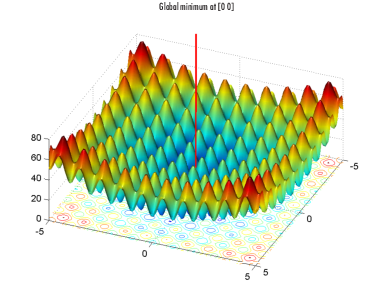
\includegraphics[width=.5\linewidth]{rastrigins_with_line2}
\end{center}

For this kind of problem:
\begin{itemize}
\item An individual is of course a (x,y) position
\item A random individual consists in random (x,y) values in [-5,5]
\item The evaluation function is $f(x,y)$
\item Crossing two individuals consists in computing intermediary values: $x_{\text{new}} = \alpha x_1 + (1-\alpha) x_2$ where $\alpha$ is a random number in $[0,1]$
\item Mutating an individual is slightly changing its (x,y) values with a random number
\end{itemize}

\subsubsection{The traveling salesman problem}

Like the Tower of Hanoi, the TSP is a classical mathematical problem. We assume a salesman has to go in various cities to sell his stuff. Plane tickets are of course at a different price to go from one city to another (or maybe there is not always a direct plane from A to B). The goal is to find the sequence of cities that will have the salesman go only once in each city, come back at his initial city, and all that with the minimum price.

In our case, the ECN administration forgot to give you the diplomas at the end of the master. I thus have to go to all students's capital cities to deliver it and of course I do not want to spend too much on the plane tickets. The file \texttt{tsp.yaml} gives the list of all cities and their distances\footnote{Plane tickets price are not proportional to distances but it was easy to generate automatically all distances between the cities}.

In this instance of Genetic algorithm:
\begin{itemize}
\item An individual is a sequence of numbers from 1 to N giving the travel ordering
\item A random individual consists in a random permutation of [1..N]
\item The evaluation function of an individual is the price required to travel through the corresponding city ordering
\item Crossing two travels consists in keeping the beginning of the first parent up to a random city, and finish with the remaining cities in the ordering given by the second parent
\item Mutating an individual can be switching two cities randomly
\end{itemize}

 \begin{itemize}
 \involves{Yaml file input}
 \end{itemize}





\end{document}
